\section{Исходные данные}
\addcontentsline{toc}{section}{Исходные данные}	% Добавляем его в оглавление

\begin{figure}[h]
  \begin{minipage}[h]{0.45\linewidth}
    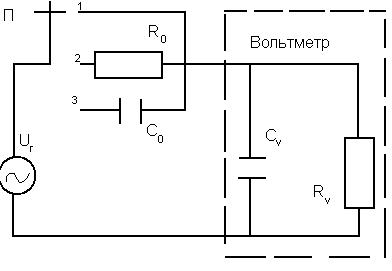
\includegraphics[width=1\linewidth]{scheme1}
    \caption{Электрическая схема ПТ с управляющим p-n-переходом с ОИ}
  \end{minipage}
  \hfill   
  \begin{minipage}[h]{0.45\linewidth}
    \vspace{4mm}
    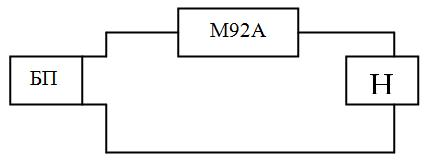
\includegraphics[width=1\linewidth]{scheme2}
    \caption{Электрическая схема МДП-транзистора с индуцированным каналом с ОИ}
  \end{minipage}   
\end{figure}

\begin{table} [htbp]
  \caption{Паспортные данные ПТ с управляющим p-n-переходом с ОИ}
  \begin{tabular}{| p{2.7cm} | p{2.7cm} | p{2.7cm} | p{2.7cm} | p{2.7cm}l | }
    \hline
    \centering Канал транзистора & 
    \centering $ S $, мА/В & 
    \centering $ U_{\text{ЗИ ПОР}} $, В &
    \centering $ P_{max} $, мВт & 
    \centering $ I_{c, max} $, мА &
    \\
    \hline
    & & & & & \\
    \hline
  \end{tabular}
\end{table}

\begin{table} [htbp]
  \caption{Паспортные данные МДП-транзистора с индуцированным каналом с ОИ}
  \begin{tabular}{| p{2.7cm} | p{2.7cm} | p{2.7cm} | p{2.7cm} | p{2.7cm}l | }
    \hline
    \centering Канал транзистора & 
    \centering $ S $, мА/В & 
    \centering $ U_{\text{ЗИ ПОР}} $, В &
    \centering $ P_{max} $, мВт & 
    \centering $ I_{c, max} $, мА &
    \\
    \hline
    & & & & & \\
    \hline
  \end{tabular}
\end{table}



\clearpage